\documentclass[a4paper,11pt]{article}
\usepackage{amsmath,amsthm,amsfonts,amssymb,amscd,amstext,vmargin,graphics,graphicx,tabularx,multicol} 
\usepackage[francais]{babel}
\usepackage[utf8]{inputenc}  
\usepackage[T1]{fontenc} 
\usepackage{pstricks-add,tikz,tkz-tab,variations}
\usepackage[autolanguage,np]{numprint} 

\setmarginsrb{1.5cm}{0.5cm}{1cm}{0.5cm}{0cm}{0cm}{0cm}{0cm} %Gauche, haut, droite, haut
\newcounter{numexo}
\newcommand{\exo}[1]{\stepcounter{numexo}\noindent{\bf Exercice~\thenumexo} : \marginpar{\hfill /#1}}
\reversemarginpar


\newcounter{enumtabi}
\newcounter{enumtaba}
\newcommand{\q}{\stepcounter{enumtabi} \theenumtabi.  }
\newcommand{\qa}{\stepcounter{enumtaba} (\alph{enumtaba}) }
\newcommand{\initq}{\setcounter{enumtabi}{0}}
\newcommand{\initqa}{\setcounter{enumtaba}{0}}

\newcommand{\be}{\begin{enumerate}}
\newcommand{\ee}{\end{enumerate}}
\newcommand{\bi}{\begin{itemize}}
\newcommand{\ei}{\end{itemize}}
\newcommand{\bp}{\begin{pspicture*}}
\newcommand{\ep}{\end{pspicture*}}
\newcommand{\bt}{\begin{tabular}}
\newcommand{\et}{\end{tabular}}
\renewcommand{\tabularxcolumn}[1]{>{\centering}m{#1}} %(colonne m{} centrée, au lieu de p par défault) 
\newcommand{\tnl}{\tabularnewline}

\newcommand{\trait}{\noindent \rule{\linewidth}{0.2mm}}
\newcommand{\hs}[1]{\hspace{#1}}
\newcommand{\vs}[1]{\vspace{#1}}

\newcommand{\N}{\mathbb{N}}
\newcommand{\Z}{\mathbb{Z}}
\newcommand{\R}{\mathbb{R}}
\newcommand{\C}{\mathbb{C}}
\newcommand{\Dcal}{\mathcal{D}}
\newcommand{\Ccal}{\mathcal{C}}
\newcommand{\mc}{\mathcal}

\newcommand{\vect}[1]{\overrightarrow{#1}}
\newcommand{\ds}{\displaystyle}
\newcommand{\eq}{\quad \Leftrightarrow \quad}
\newcommand{\vecti}{\vec{\imath}}
\newcommand{\vectj}{\vec{\jmath}}
\newcommand{\Oij}{(O;\vec{\imath}, \vec{\jmath})}
\newcommand{\OIJ}{(O;I,J)}


\newcommand{\reponse}[1][1]{%
\multido{}{#1}{\makebox[\linewidth]{\rule[0pt]{0pt}{20pt}\dotfill}
}}

\newcommand{\titre}[5] 
% #1: titre #2: haut gauche #3: bas gauche #4: haut droite #5: bas droite
{
\noindent #2 \hfill #4 \\
#3 \hfill #5

\vspace{-1.6cm}

\begin{center}\rule{6cm}{0.5mm}\end{center}
\vspace{0.2cm}
\begin{center}{\large{\textbf{#1}}}\end{center}
\begin{center}\rule{6cm}{0.5mm}\end{center}
}



\begin{document}
\pagestyle{empty}
\titre{{\Large Le petit truc en plus}}{Nom :}{Prénom :}{3ème}{}


\vspace*{1cm}



\begin{flushright}

\textit{\textbf{{\large A rendre avant le  vendredi 26 octobre !}}}

\end{flushright}


\vspace*{1cm}

\exo \\
Benoît a construit une armoire de 2,10 m
de hauteur et de 0,70 m de profondeur
dans sa chambre. Il décide de la relever
pour l'installer.\\
Sa chambre mesure 2,20 m de hauteur.
Pourra-t-il la lever ? (Justifier votre réponse)

\begin{center}
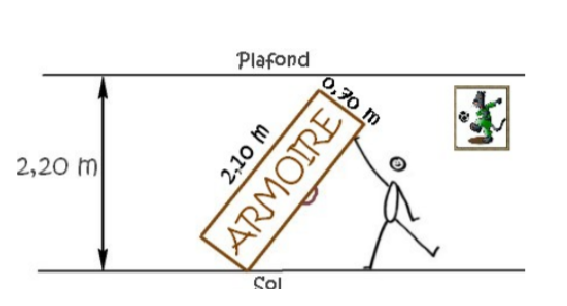
\includegraphics[scale=1]{Armoire.eps} 
\end{center}
\vspace*{1cm}

\exo \\
Philippe le Bel est monté sur le trône de France en 1285. Ses trois fils ont régné après lui : Louis X le
Hutin, Philippe V le Long et Charles IV le Bel.\\

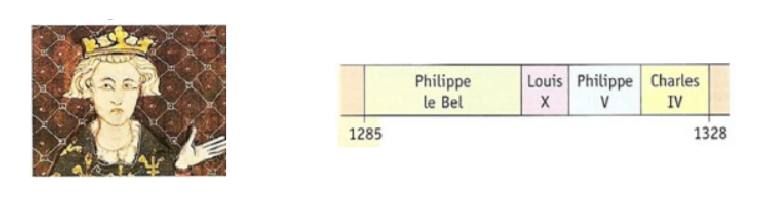
\includegraphics[scale=1]{histoire.eps} \\

\noindent - Louis X a régné 27 ans de moins que son père.\\
- Le règne de Philippe V a été trois fois plus long que celui de Louis X.\\
- Charles IV a été roi pendant le même nombre d'années que Philippe V.\\



\initq \q On note x la durée, en années, du règne de Louis X. Écrire en fonction de x la somme des règnes des
quatre rois.\\
\q  Le règne de Louis X a été court. A-t-il duré 1 an, 2 ans ou 5 ans ?\\
En déduire la durée des règnes des trois autres rois.\\

\vspace*{1cm}

\exo \\
Un ouvrier met 8 jours pour creuser un trou de 8 m de long sur 8 m de large et profond de 8 m.
Combien de jour mettra-t-il pour creuser un trou de 4 m de long sur 4 m de large et profond de 4 m ? (Justifier votre réponse)




\vspace*{1cm}

\begin{flushright}
\fbox{{\LARGE \textbf{NOTE} : . . . /10}  }
\end{flushright}

\end{document}
